\onecolumn
\setcounter{equation}{0}
\renewcommand\theequation{A.\arabic{equation}}
\section*{Appendix}
\label{sec:appendix}
\subsubsection*{Decomposition of MSE in bias and variance}
\begin{align}\label{eq:derivation_bias_variance}
\begin{split}
	\mathds{E}[(y-\tilde{y})^2] =& \mathds{E}[(f+\epsilon - \tilde{y})^2] \\
	=& \mathds{E}[\left(f+\epsilon - \tilde{y} + \mathds{E}[\tilde{y}] - \mathds{E}[\tilde{y}]\right)^2] \\
	=& \mathds{E}[(f-\mathds{E}[\tilde{y}])^2] + \mathds{E}[\epsilon^2] + \mathds{E}[(\mathds{E}[\tilde{y}]-\tilde{y})^2] + 2\mathds{E}[(f-\mathds{E}[\tilde{y}])\epsilon] \\
	&+ 2\mathds{E}[\epsilon(\mathds{E}[\tilde{y}]-\tilde{y})] + 2\mathds{E}[(\mathds{E}[\tilde{y}]-\tilde{y})(f-\mathds{E}[\tilde{y}])] \\
	=& (f-\mathds{E}[\tilde{y}])^2 + \mathds{E}[\epsilon^2] + \mathds{E}[(\mathds{E}[\tilde{y}]-f)^2] + 2(f-\mathds{E}[\tilde{y}])\mathds{E}[\epsilon] \\
	&+ 2\mathds{E}[\epsilon]\mathds{E}[\mathds{E}[\tilde{y}]-\tilde{y}] + 2\mathds{E}[\mathds{E}[\tilde{y}]-\tilde{y}](f-\mathds{E}[\tilde{y}]) \\
	=& (f-\mathds{E}[\tilde{y}])^2 + \mathds{E}[\epsilon^2] + \mathds{E}[(\mathds{E}[\tilde{y}]-\tilde{y})^2] \\
	=& Bias[\tilde{y}]^2 + Var[y] + Var[\tilde{y}] \\
	=& Bias[\tilde{y}]^2 + \sigma^2 + Var[\tilde{y}]
\end{split}
\end{align}
Here, we have used that
\begin{equation*}
	\mathds{E}[X^2] = Var[X] + \left(\mathds{E}[X]\right)^2
\end{equation*}
\begin{equation*}
	\mathds{E}[f]=f \rightarrow \mathds{E}[y]=\mathds{E}[f+\epsilon] = f
\end{equation*}
\begin{equation*}
	Var[\epsilon] = \sigma^2 \rightarrow Var[y] = \mathds{E}[(f+\epsilon-f)^2] = \sigma^2
\end{equation*}

\subsubsection*{Visualization of terrain data}
Figure \ref{fig:terrainpic} visualizes the real terrain data before reduction. Figure \ref{fig:terrainpic_reduced} displays the data after reduction, for comparison.

\begin{figure}[htbp]
	\centering
	\begin{subfigure}{.5\textwidth}
		\centering
		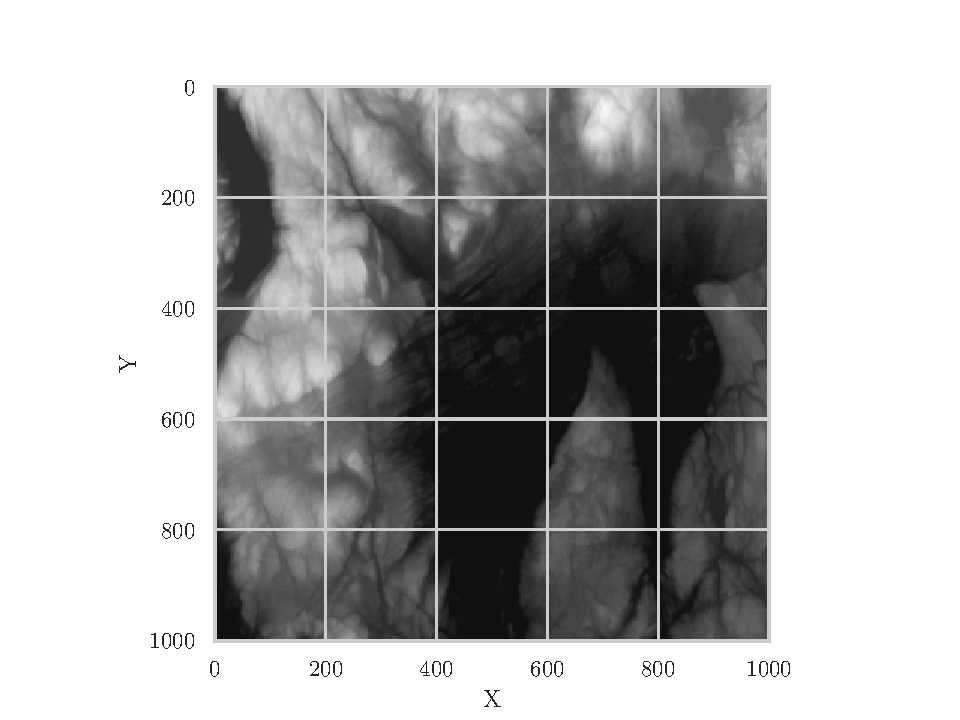
\includegraphics[width=\linewidth]{terrainpicture.pdf}
		\caption{Full terrain data over the Inner \\Oslo fjord with $1000\times 1000$ data points. \\Here black represents the ocean level.}
		\label{fig:terrainpic}
	\end{subfigure}%
	\begin{subfigure}{.5\textwidth}
		\centering
		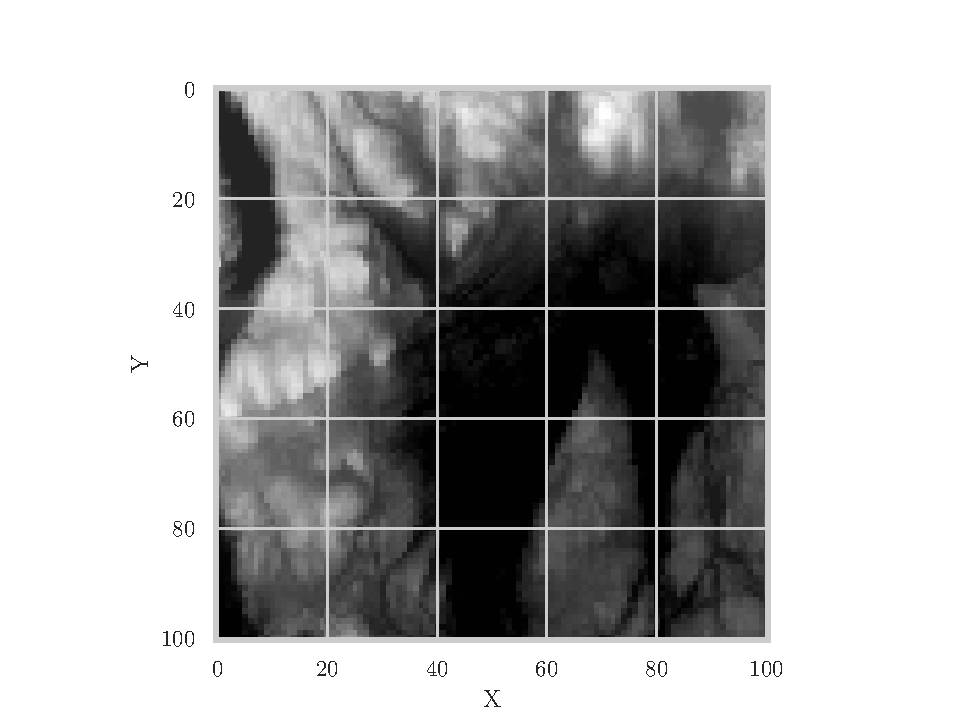
\includegraphics[width=\linewidth]{terrainpicture_reduced.pdf}
		\caption{Reduced terrain data over the Inner Oslo fjord in grey scale with $100\times 100$ data points, i.e. every tenth point of every tenth row of the full data set.}
	\label{fig:terrainpic_reduced}
	\end{subfigure}
	\caption{Comparison of full and reduced terrain data. As geographical reference, Nesoddtangen can be seen to the lower right, with Bunnefjorden to the right and the Inner Oslo fjord in the centre. Parts of Drammensfjorden can be seen to the far left.}
	\label{fig:terrain}
\end{figure}

\begin{figure}[htbp]
\centering
\label{fig:franke_visual}
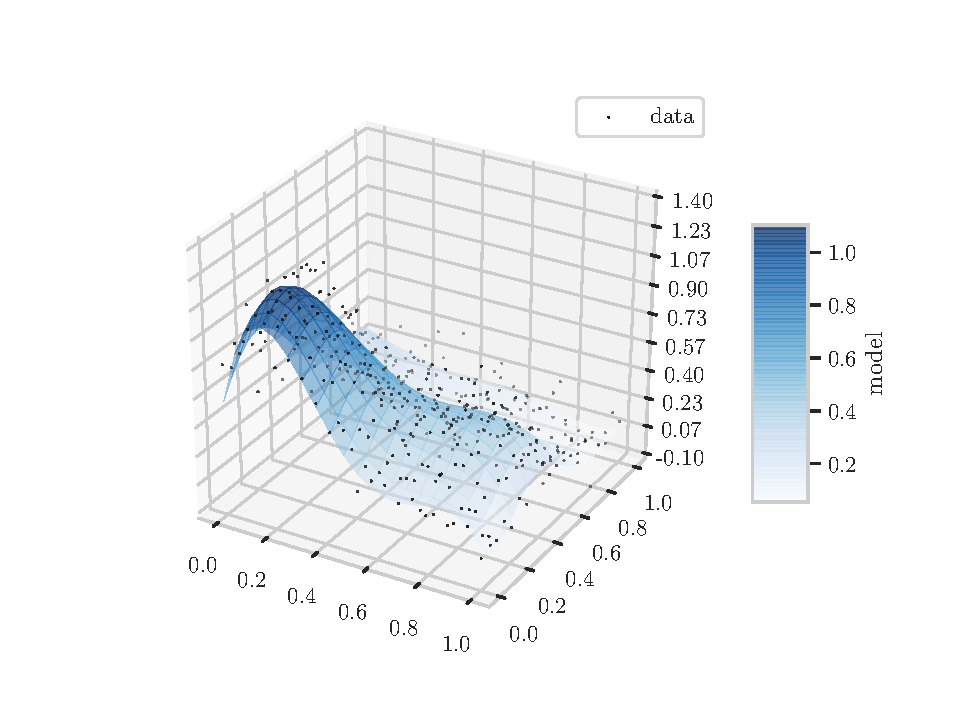
\includegraphics[width=0.5\textwidth]{../figures/franke_visual}
	\caption{The prediction $z$ produced by OLS on Frankes function with a polynomial of degree $m=5$. Det scatter plot is the data, and the surface plot is the predicted model.}
\end{figure}

\begin{figure}[htbp]
\centering
\label{fig:terrainpic_ridge}
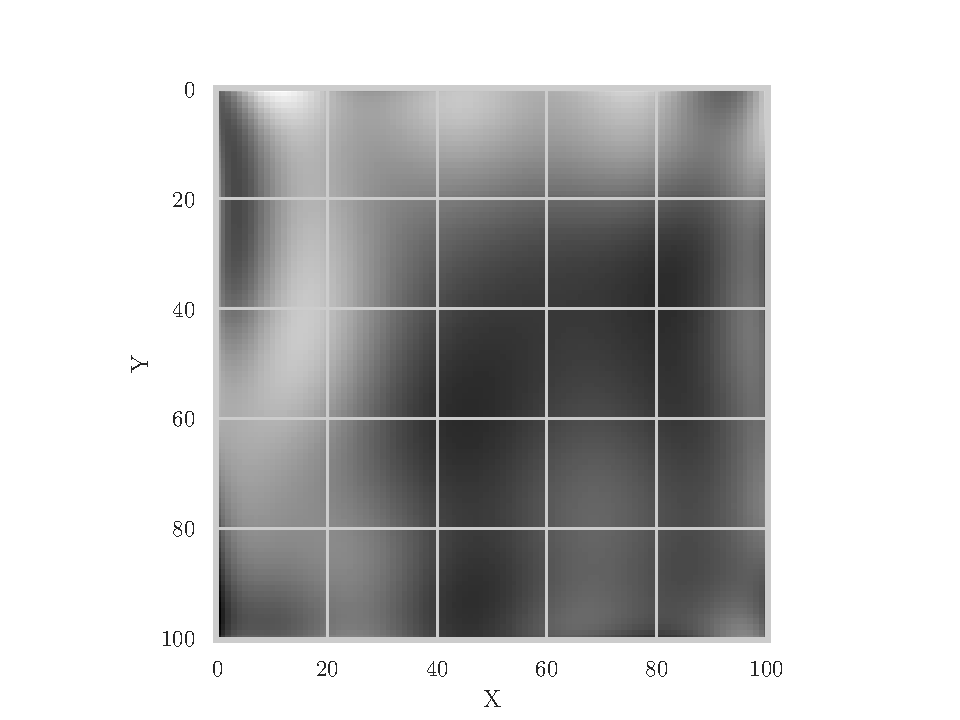
\includegraphics[width=0.5\textwidth]{../figures/terrainpicture_ridge}
	\caption{The prediction $z$ produced by ridge regression with polynomial of degree $m=10$.}
\end{figure}

%  \[A =
%    \mqty[b_1 & c_1 & 0 & \hdots & \hdots & 0 \\
%          a_1 & b_2 & c_2 & 0 & \hdots & 0 \\
%          0 & a_2 & b_3 & c_3 & \hdots & 0 \\
%          \vdots & \ddots & \ddots & \ddots & \ddots & \vdots \\
%          0 & \hdots & \ddots & a_{n-2} & b_{n-1} & c_{n-1} \\
%          0 & \hdots & \hdots & 0 & a_{n-1} & b_n],
%  \]
